\qrchapter{https://forgottenpillar.com/rsc/en-fp-chapter1}{The historical context}

\qrchapter{https://forgottenpillar.com/rsc/en-fp-chapter1}{Muktadha wa kihistoria}

Ellen White alikumbuka kukutana na maoni yale yale katika \textit{The Living Temple} ambayo alikuwa ameonywa dhidi yake katika huduma yake ya awali:

\egw{Tulipokuwa tunasoma \normaltext{[The Living Temple]}, nilitambua maoni yale yale ambayo nilikuwa nimeamriwa kuaongea dhidi yao kwa onyo \textbf{wakati wa siku za mwanzo za kazi yangu ya hadhara}. \textbf{Nilipotoka kwanza \underline{Jimbo la Maine, ilikuwa ni kupitia Vermont na Massachusetts}}, kubeba ushuhuda \textbf{dhidi ya maoni haya}. ‘Living Temple’ ina alfa ya nadharia hizi. Nilijua kwamba omega ingefuata baada ya muda mfupi; na nilitetemeka kwa ajili ya watu wetu. Nilijua kwamba nilihitaji kuwaonya ndugu na dada zetu \textbf{wasijihusishe na mgogoro juu ya \underline{uwepo na umbile la Mungu}}. Taarifa zilizotolewa katika ‘Living Temple’ kuhusiana na nukta hii si sahihi. Maandiko yaliyotumika kuthibitisha mafundisho yaliyowekwa hapo, ni maandiko yaliyotumika vibaya.}[SpTB02 53.2; 1904][https://egwwritings.org/read?panels=p417.271]

Alitaja kukutana kwake kwa mara ya kwanza na maoni haya: \egwinline{Nilipotoka kwanza \textbf{Jimbo la Maine}, ilikuwa ni kupitia Vermont na Massachusetts, \textbf{kubeba ushuhuda dhidi ya maoni haya.}} Wasifu wake, ulioandikwa na mjukuu wake Arthur Lacey White, unatoa muktadha zaidi kuhusu maoni haya. Katika \textit{Ellen White: The Early Years}, chini ya sehemu \textit{Wrestling with the Views of the Spiritualizers}, uzoefu wake katika mashariki ya Maine unafunua zaidi kuhusu mgogoro juu ya umbile la Mungu na maana zake.

\othersQuote{\textbf{\underline{Katika mashariki ya Maine} Ellen alikuwa akisafiri} na kufanya kazi \textbf{katika mazingira ya wale wanaofasiri mambo kiroho, ambao walikuwa \underline{wamefanya mbingu, Mungu, Yesu, na tumaini la Ujio kuwa mafumbo}}. Katika maono huko Exeter katikati ya Februari alionekana \textbf{kuwa katika uwepo wa Yesu, na alikuwa na hamu ya kupata majibu ya baadhi ya \underline{maswali muhimu}}.}[ALW, 1BIO 79.4; 1985][https://egwwritings.org/read?panels=p668.582]

\othersQuoteNoGap{Nilimwuliza Yesu kama \textbf{Baba yake alikuwa na umbo kama Yeye}. \textbf{Akasema alikuwa nalo}, lakini sikuweza kuliona, kwani alisema, ‘Kama ungaliona mara moja utukufu wa \textbf{Umbile Lake}, ungekoma kuwepo.’—Early Writings, 54.}[ALW, 1BIO 79.5; 1985][https://egwwritings.org/read?panels=p668.583]

\othersQuoteNoGap{Hii haikuwa tukio la pekee ambapo Ellen aliongea na Yesu na malaika \textbf{kuhusu \underline{nafsi ya Yesu} na kuhusu \underline{Mungu kuwa nafsi binafsi}}. \textbf{\underline{Majibu yalimridhisha kabisa kwamba wale wanaofasiri mambo kiroho walikuwa katika makosa makubwa}}.}[ALW, 1BIO 80.1; 1985][https://egwwritings.org/read?panels=p668.586]

Maono ambayo Arthur Lacey White aliyarejea yanajulikana kama \textit{maono juu ya umbile la Mungu}, ambayo tutayachunguza baadaye. Maono haya yanathibitisha kwamba fundisho la \emcap{umbile la Mungu} linafundisha kwamba Mungu Baba ana umbo, kama vile Yesu alivyo. Inaelezea hasa kuhusu \others{\textbf{nafsi ya Yesu} na kuhusu \textbf{Mungu kuwa nafsi binafsi}.}

\begin{figure}[t]
    \centering
    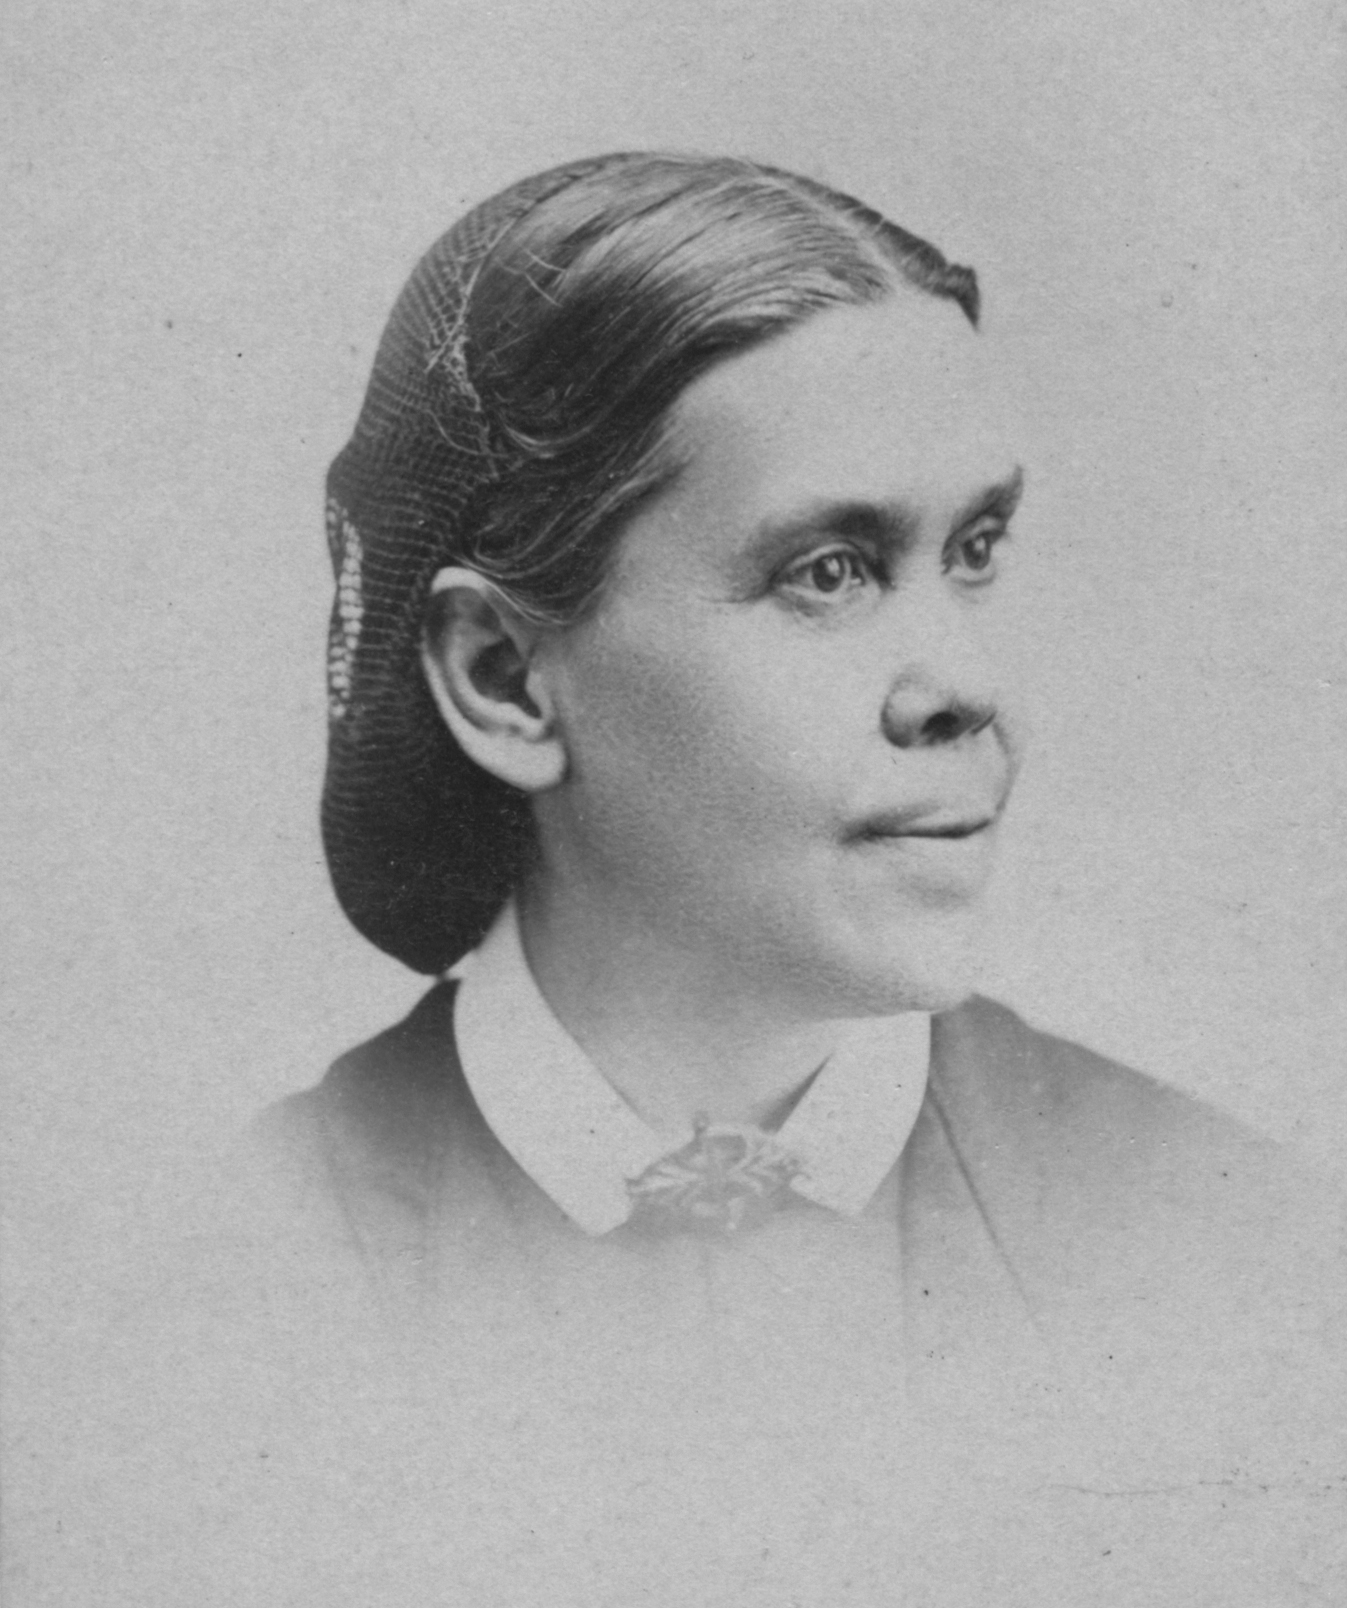
\includegraphics[width=0.65\linewidth]{images/ellen-white.jpg}
    \caption*{Ellen G. White}
    \label{fig:ellen-g-white}
\end{figure}

\begin{figure}[t]
    \centering
    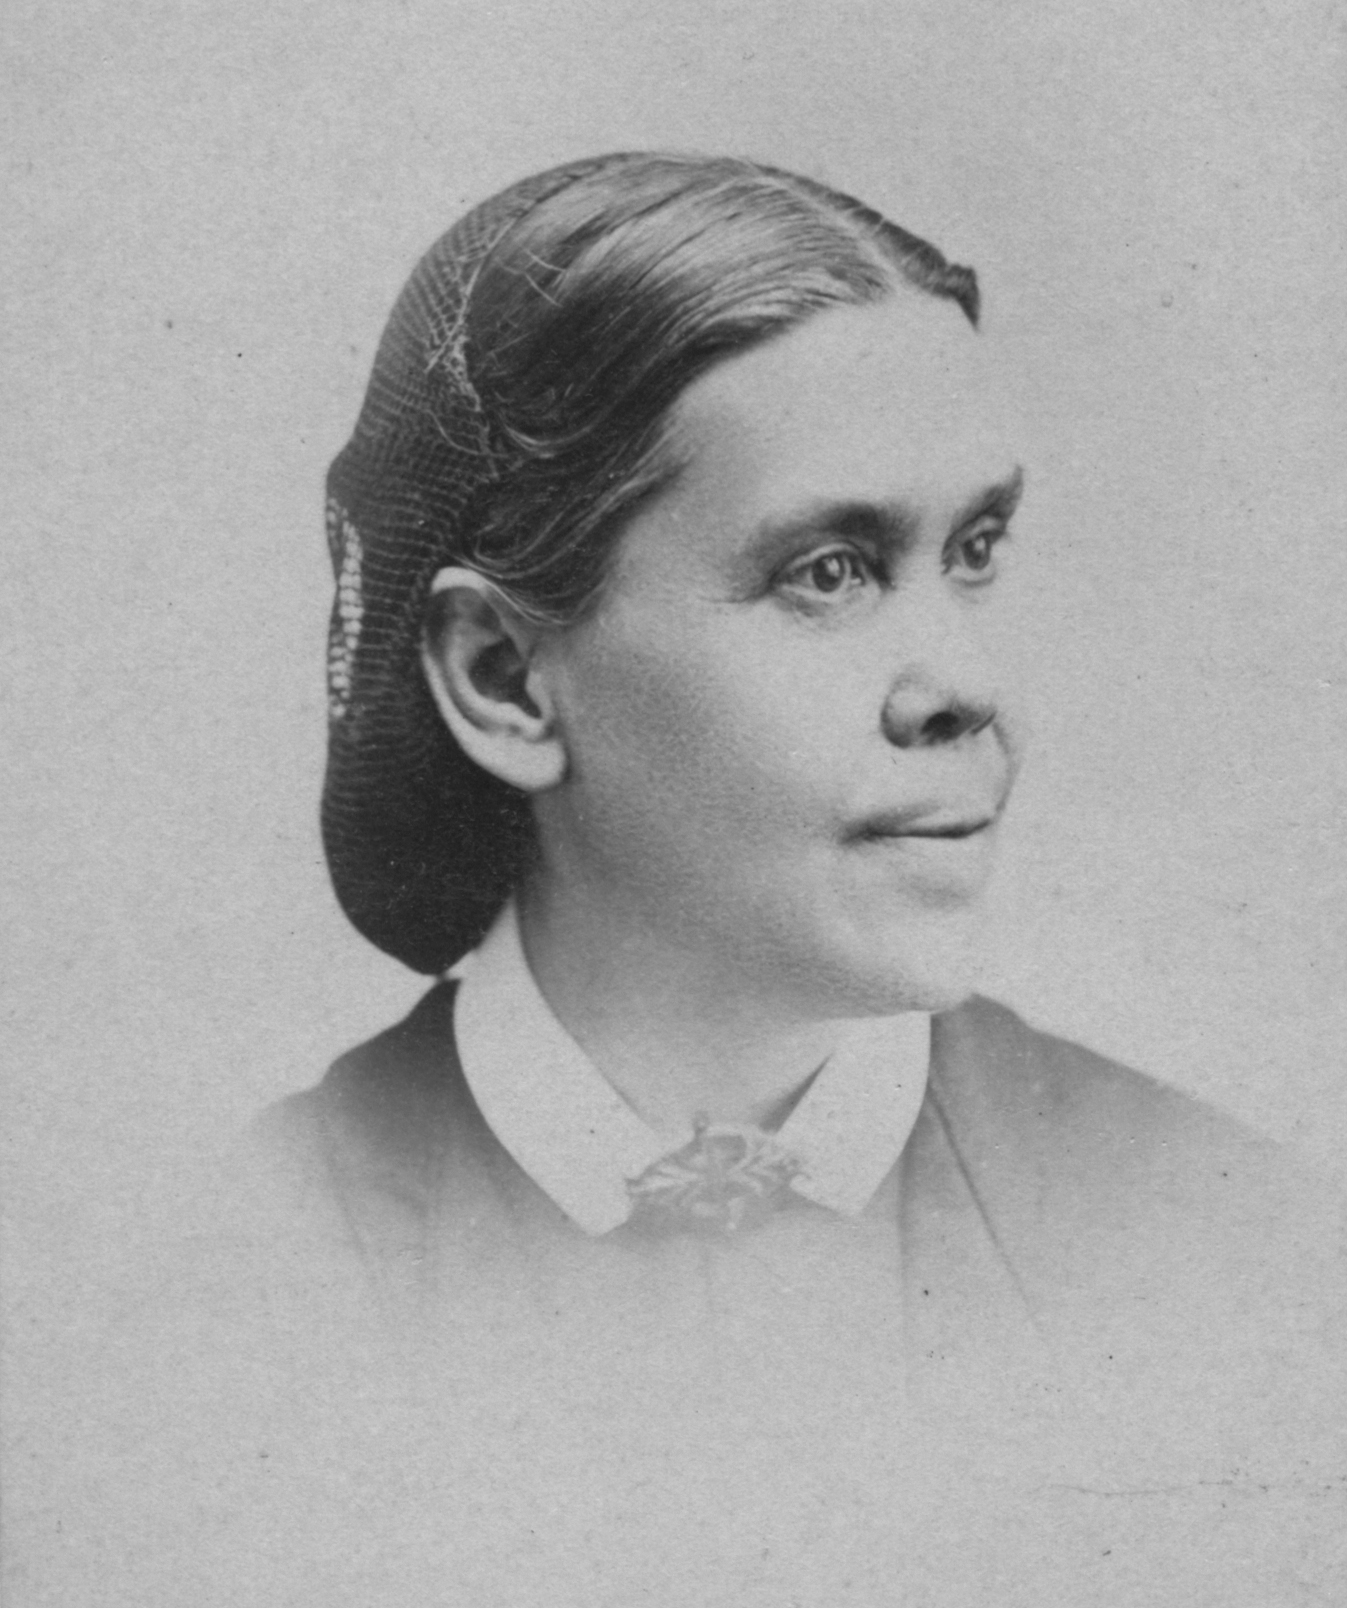
\includegraphics[width=0.65\linewidth]{images/ellen-white.jpg}
    \caption*{Ellen G. White}
    \label{fig:ellen-g-white}
\end{figure}

Fikiria nukta ya kwanza ya \emcap{Kanuni za Kimsingi}, ambayo inasema kwamba Waadventista Wasabato wanaamini katika \others{Mungu mmoja, \textbf{nafsi binafsi, wa kiroho}.}[First point of the Fundamental Principles][https://forgotten-pillar.s3.us-east-2.amazonaws.com/A+declaration+of+the+fundamental+principles+taught+and+practiced+by+the+Seventh-day+Adventists++.pdf] Hii inafanya iwe wazi kwamba suala kuu katika fundisho la \emcap{umbile la Mungu} linahusu umbo la nje, la kimwili la Baba. Lakini kwa nini hili lilikuwa swali muhimu na la maana sana? Nini maana ya Mungu kuwa na umbo la kimwili, la kibinafsi?

\othersQuote{Lakini kwa sababu waanzilishi wa Kanisa la Waadventista Wasabato walishikilia kwamba unabii ulitimizwa Oktoba 22, 1844, na kwamba kazi muhimu ilianza mbinguni katika Patakatifu pa Patakatifu pa hekalu la mbinguni wakati huo, na kwa sababu Waadventista ambao walikuwa wamekuwa \textbf{wanarohanishaji} walichukua msimamo kwamba Kristo alikuwa amekuja ndani ya mioyo yao Oktoba 22, 1844, na kwamba Ufalme wake ulikuwa ndani ya mioyo yao, waanzilishi wa kanisa, na hasa Ellen White, waliwekwa na ulimwengu kwa ujumla na wale, na vilevile wale ambao Waadventista Wasabato wamewataja kama Waadventista wa siku ya kwanza waliwaweka kama kundi moja na lilelile. Hapa tena adui mkuu alitupa shutuma juu ya ukweli, akiulinganisha na uzoefu wa uongo na bandia.}[ALW, 1BIO 80.2; 1985][https://egwwritings.org/read?panels=p668.587]

\othersQuoteNoGap{Ellen White alikuwa azungumzie jambo hili tena, hasa katika aya za mwisho za kitabu chake cha kwanza kifupi, Experience and Views, kilichochapishwa mwaka 1851. Mtu anapoisoma hii ataona matumizi ya \textbf{neno umizimu}, ambalo lazima lichukuliwe katika mwanga wa kazi ya wanarohanishaji na sio katika mwanga wa kile ambacho leo kinafahamika kuwa umizimu au ushetani, ingawa vyote vinatoka kwenye chanzo kilekile kimoja.}[ALW, 1BIO 80.3; 1985][https://egwwritings.org/read?panels=p668.588]

\othersQuoteNoGap{Sasa tunageukia taarifa iliyoandikwa na kuchapishwa mwaka 1851 kama inavyopatikana katika Ibid., 77, 78:}[ALW, 1BIO 80.4; 1985][https://egwwritings.org/read?panels=p668.589]

\othersQuoteNoGap{\textbf{Mara nyingi nimeshtakiwa kwa uongo kwa kufundisha maoni yanayofanana na Umizimu}. Lakini kabla mhariri wa The Day-Star hajaingia katika upotovu huo, \textbf{Bwana \underline{alinipa maono} ya matokeo ya kusikitisha na ya kuharibu ambayo yangezalishwa juu ya kundi na yeye pamoja na wenzake  wengine \underline{katika kufundisha maoni ya kiroho}}.}[ALW, 1BIO 80.5; 1985][https://egwwritings.org/read?panels=p668.590]

\othersQuoteNoGap{Mara nyingi nimemwona \textbf{Yesu aliye mwema na mzuri, kwamba Yeye ni Nafsi}. Nilimwuliza \textbf{\underline{kama Baba yake alikuwa Nafsi} na \underline{alikuwa na umbo} kama Yeye}. Yesu alisema, ‘Mimi ni \textbf{chapa kamili ya Umbile Wake}.}[ALW, 1BIO 80.6; 1985][https://egwwritings.org/read?panels=p668.591]

\othersQuoteNoGap{\textbf{Mara nyingi nimeona kwamba \underline{mtazamo wa kiroho} uliondoa utukufu wote wa mbinguni, na kwamba katika akili nyingi kiti cha enzi cha Daudi na nafsi nzuri ya Yesu zimeteketezwa katika moto wa Umizimu.} Nimeona kwamba baadhi ya wale ambao wamedanganywa na kuongozwa katika kosa hili wataletwa nje katika nuru ya ukweli, lakini itakuwa haiwezekani kwa urahisi kwao kuondokana kabisa na \textbf{nguvu ya udanganyifu wa Umizimu}. Watu kama hao wanapaswa kufanya kazi ya kina katika kukiri makosa yao na kuyaacha milele.}[ALW, 1BIO 80.7; 1985][https://egwwritings.org/read?panels=p668.592]

\othersQuoteNoGap{\textbf{Urohanishaji wa mbinguni, Mungu, Kristo, na kuja kwa Kristo ulikuwa katika msingi wa mafundisho mengi ya ushupavu ambayo Ellen Harmon mwenye umri wa miaka 17 aliitwa na Mungu kukabiliana nayo katika siku hizo za mwanzo. Maono yaliimarisha kwa dhati \underline{Umbile la Mungu na Kristo}, \underline{uhalisia wa mbinguni} na thawabu kwa waaminifu, na ufufuo. Mwongozo huu thabiti uliokoa kanisa linalojitokeza}.}[ALW, 1BIO 81.1; 1985][https://egwwritings.org/read?panels=p668.595]

Kosa la harakati ya Millerite mwaka 1844 lilikuwa katika kutoeleweka kwa asili ya tukio, sio wakati wake. Danieli 7:13-14 inaelezea Kristo akija kwa Mzee wa Siku mbinguni kupokea mamlaka, utukufu, na ufalme—sio kuja kwake mara ya pili duniani. Tukio hili, likiashiria mwanzo wa kazi ya Kristo katika Patakatifu pa Patakatifu, lilitokea mwishoni mwa unabii wa siku 2300 mwaka 1844. Tofauti na makundi mengine ya Waadventista, Kanisa la Waadventista Wasabato lililojitokeza lilikuwa pekee kutambua tukio hili la mbinguni.

Uelewa huu umejengwa juu ya misingi muhimu:
\begin{itemize}
    \item Mbingu ni mahali halisi, la kawaida (Yohana 14:1-3).
    \item Kuna patakatifu halisi mbinguni ambapo Kristo anahudumu (Waebrania 8:2). 
    \item Kiti cha enzi halisi, cha kimwili kipo katika patakatifu hili, kinachokaliwa na Mungu Mwenyewe (Danieli 7:9-10; Ufunuo 4:2-3; Ezekieli 1:26-28; Zaburi 11:4).
\end{itemize}

Kwa nini swali la umbo la kimwili la Baba ni muhimu sana? Kama Mungu asingekuwa kiumbe cha kimwili, kusingekuwa na haja ya kiti cha enzi halisi, patakatifu, au huduma ya mbinguni. Tafsiri ya kiroho inapunguza msingi wa theolojia ya Waadventista Wasabato, na kusababisha athari ya domino inayoharibu fundisho la kazi ya ukuhani ya Kristo.

Fundisho la \emcap{Umbile la Mungu} lilikuwa mafundisho rahisi lakini ya msingi, lililothibitishwa katika nukta ya kwanza ya \emcap{Kanuni za Kimsingi}: \textit{“Mungu Mmoja, Nafsi Binafsi wa kiroho.”} Kwa hivyo, Yeye si mwenye kuwepo kila mahali kwa Nafsi Yake bali kupitia Mwakilishi Wake, Roho Mtakatifu.\footnote{Nukta ya kwanza ya Kanuni za Kimsingi: \othersQuote{Kwamba kuna \textbf{Mungu mmoja}, \textbf{\underline{Nafsi Binafsi wa kiroho}}, muumba wa vitu vyote, mwenye uwezo wote, … na \textbf{yupo kila mahali kupitia \underline{mwakilishi wake}, Roho Mtakatifu}. Zab. 139:7.}} Wakati Ellen White alipomuuliza Yesu \egwinline{kama Baba Yake \textbf{alikuwa Nafsi} na \textbf{alikuwa na \underline{umbo}} kama Yeye Mwenyewe,}[EW 77.1; 1882][https://egwwritings.org/read?panels=p28.490&index=0] tunaona wazi kwamba \textit{umbo la nje la mwili} ni \textit{ubora au hali} inayomfafanua Mungu kama Nafsi. Uelewa huu ulikuwa muhimu katika kushughulikia mgogoro wa Kellogg kuhusu \textit{The Living Temple}, ambayo ilikengeuka kutoka imani hii ya msingi.

Lakini je, \textit{Mafundisho za Kimsingi} zetu za sasa bado zinathibitisha fundisho hili? Je, zinafundisha wazi kwamba Mungu ni Nafsi halisi mwenye umbo la kimwili, ambaye uwepo wake halisi uko mbinguni, wakati Yeye yupo kila mahali kupitia Roho Wake? Fundisho la uwepo na Umbile la Mungu halipo katika imani rasmi za leo. Ingawa kila mmoja wetu, tunaweza bado kuamini ndani yake, kwa nini mafundisho muhimu kama hayo yaliachwa? Zilikuwa sababu gani zilizosababisha mabadiliko haya? Haya ndio maswali ambayo lazima tuchunguze zaidi katika muktadha wa \textit{Msingi wa Imani Yetu}.

% The Historical Context

\begin{titledpoem}
    
    \stanza{
        By visions Ellen White stood firm, \\
        Against false views; she did affirm. \\
        The Father’s form, a truth profound, \\
        In this essential faith was found.
    }

    \stanza{
        "Spiritualizers" sought to claim \\
        That heaven’s realm was but a name. \\
        Yet God has form, like Christ His Son, \\
        This truth our founders built upon.
    }

    \stanza{
        A Spirit Person God does reign \\
        The universe is His domain \\
        This doctrine once our cornerstone, \\
        Has somehow from our statements flown.
    }
    
\end{titledpoem}

% The Historical Context

\begin{titledpoem}
    
    \stanza{
        By visions Ellen White stood firm, \\
        Against false views; she did affirm. \\
        The Father’s form, a truth profound, \\
        In this essential faith was found.
    }

    \stanza{
        "Spiritualizers" sought to claim \\
        That heaven’s realm was but a name. \\
        Yet God has form, like Christ His Son, \\
        This truth our founders built upon.
    }

    \stanza{
        A Spirit Person God does reign \\
        The universe is His domain \\
        This doctrine once our cornerstone, \\
        Has somehow from our statements flown.
    }
    
\end{titledpoem}
